%%%%%%%%%%%%%%%%%%%%%%%%%%%%%
%Since : 2018/11/13
%Update: <2019/03/01>
% -*- coding: utf-8 -*-
%%%%%%%%%%%%%%%%%%%%%%%%%%%%%
\documentclass[12pt, a4j]{jreport}
\usepackage[dvipdfmx]{graphicx}
%\usepackage{graphicx}
\usepackage{amsmath}
\usepackage{amssymb}
\usepackage{cite}

\renewcommand{\prechaptername}{第}
\renewcommand{\postchaptername}{回}
\renewcommand{\thesection}{\arabic{section}}

\title{Excelによる統計処理実習}
\author{公立小松大学臨床工学科 \\ 藤田 一寿}
\date{}

\begin{document}

\maketitle

\chapter{Excelによる統計処理1}

\section{目的}

Excelの操作を通し,データ処理の基礎とグラフの作成の仕方を学ぶ.

\section{理論}

\subsection{統計とは}


全体の特徴を捉える.

サンプル

\subsection{統計量}

総和


平均
\begin{equation}
    \mu = \frac{1}{N} \sum_{i=1}{N}
\end{equation}

中央値

分散
\begin{equation}
    \sigma^2 = \frac{1}{N} \sum_{i=1}{N} (x - \mu)^2
\end{equation}

\subsection{グラフ}

データの可視化.
視覚的理解の促進.

\paragraph{ヒストグラム}

データの分布の様子の把握に用いられる.


\paragraph{折れ線グラフ}

値の時間変化の把握に用いられる.


\paragraph{散布図}

値の関係性を見るために用いられる.


\section{Excel実験}

\subsection{総和,平均,中央値,分散}

エクセルでの総和の計算は次の手順で行う.

\begin{enumerate}
    \item 総和を表示したいセルを選択する.
    \item ``=sum(''と入力する.
    \item 総和を計算したいセルを選択する.\footnote{データを選択する方法はいくつかあります.皆さんの慣れた方法でやってください.}そうすると``(''の後ろにセル番号が入力される(図\ref{fig:sum}).
    \item )を入力する.
\end{enumerate}

\begin{figure}[htbp]
  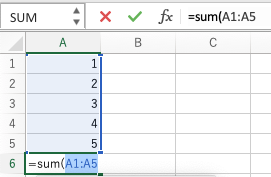
\includegraphics[width=10cm]{sum.png}
  \caption{総和を計算したいセルを選択した状態.}
  \label{fig:sum}
\end{figure}

同じやり方で,平均,分散が計算できる.平均なら``sum''の部分を``mean''.

\paragraph{演習}
csvの平均,分散を求めよ.
csvの平均,中央値を求めよ.そして,平均値と中央値の差について考察せよ.

\subsection{ヒストグラム}




\paragraph{演習}
csvをヒストグラムにせよ.


\subsection{折れ線グラフ}



\paragraph{演習}
折れ線グラフ.



\subsection{散布図}

\paragraph{演習}
散布図をかけ.



\section{考察}



\section{おまけ}

ファイル形式

確率分布

ガウス分布

不偏分散

\chapter{Excelによる統計処理2}

\section{目的}

エクセルにはデータを解析するための関数が多く用意されている.今回はその一部を用い,データ解析の初歩を学ぶ.

\section{原理}

\subsection{度数分布表とヒストグラム}

\subsection{相関係数}

\subsection{共分散}

\subsection{散布図と回帰直線}


\section{実験}

\subsection{度数分布表とヒストグラム}

\paragraph{演習}
csvデータから度数分布表を書け.

\paragraph{演習}
度数分布表に基づきヒストグラムをかけ.


\subsection{相関係数}

\paragraph{演習}
csvデータから相関係数を求めよ.

\subsection{共分散}

\paragraph{演習}
csvデータから相関係数を求めよ.

\subsection{演習}
散布図回帰直線

\paragraph{演習}

csvデータから散布図と回帰直線をかけ.


標本分散の期待値を求めよ.

\section{考察}



\section{おまけ}
R,python

プロット
R,matplotlib,gnuplot


有料ならmatlabがある.

\section{レポートの出し方}

提出は電子データで送る.データ形式はpdfもしくはdocxとする.


\end{document}
